% (c) Jakub Stejskal
% Master Thesis
% Performance Testing and Analysis of Qpid-Dispatch Router
% Chapter 4

\chapter{Analysis and Design}
\label{Analysis and Design}
Maestro is specially designed for the performance testing of the Broker. However, with the significant Qpid-Dispatch growth, the need for performance testing emerges. In the following we will analyze the Qpid-Dispatch service with focus on its capabilities and methodology. Moreover we will describe the design of the Topology Generator and Qpid-Dispatch Performance Module for Maestro, which are the main requirements to achieve the actual performance testing of Qpid-Dispatch router.

\section{Used Technologies}
The most of Maestro, such as the command parsing, reporting, clients abstractions and so on, is written in Java language. But the whole Maestro is not a pure Java code. For test specificatio we use Groovy instead. Groovy is basically a lightweight version of Java with several advantages. In particular, Groovy scripts are more readable for those who are not much familiar with Java code. Groovy scrips are also used as handlers for specific commands for extension points, which is described in more depth in the Subsection \ref{MPT Preparations}.

On the other hand, Topology Generator is a new simple project. For easy integration to another projects, quick development, and easy code preview it was developed in the \emph{Python} language. Whole generator is created as one package, which is available for installation on any machine with installed Python version 2.7 and higher. The rest of the following will describe the rest of the used technologies.

\subsection{Ansible}
Ansible \cite{Ansible} is a simple automation framework which allow users to automate daily tasks on multiple nodes or containers. Basic types of tasks which can be automated by Ansible are:

\begin{itemize}
	\item \textbf{Provisioning}\,---\,setups the various servers in the network infrastructure.
	\item \textbf{Configuration management}\,---\,changes configuration of an application, operation system or device. Basically this allows starting, stopping and restarting services, installing or updating applications or performing a wide variety of other configuration tasks.
	\item \textbf{Application deployment}\,---\,automatically deploys the internally developed application to specified systems with all dependencies.
\end{itemize}

Ansible scripts, called playbooks, are written in YAML language. This makes Ansible scripts easy to read for humans and simple to manage. Another advantage is that the user does not even need to know commands used to accomplish a particular tasks. All that is needed is to specify what state does user wants the system to be in. Ansible is available on multiple systems with really short list of dependencies; Linux based systems requires Python installed, while Windows requires PowerShell; both systems requires SSH support. Moreover, Ansible playbooks can be grouped together and create more complex scripts called roles. These are open-source and available in the public repository.

\begin{figure}[H]
  \centering
  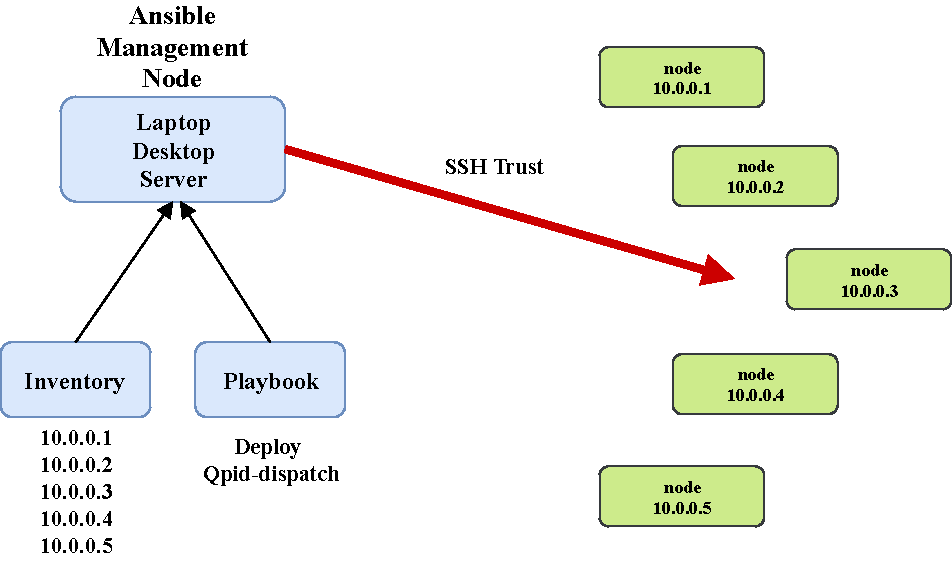
\includegraphics[width=12cm]{obrazky-figures/ansible_architecture.pdf}
  \caption{Example of Ansible architecture with several nodes. Inventory and Playbook are passed to Ansible Management node, which executes the playbook on all node specified in the inventory.}
  \label{fig:ansible_architecture}
\end{figure}

We use Ansible for several tasks; mainly to deploy systems on specific nodes. As we~want to run performance tests of Qpid-dispatch over multiple topology scenarios it is necessary to do system deployment quickly and automatically, which is easy with Ansible. System deployment contains installation of Maestro, Qpid-dispatch and other services based on the testing scenario. The next usage is to create and deploy configuration files for each router. This task runs the Topology generator and creates configuration files for each machine based on the generator output.


\subsection{Docker}
Docker \cite{Docker} is an open platform that provides developing, shipping, and running application separately from the infrastructure. Basically Docker is a specific type of virtualization technology. It allows to package and run an application in a loosely isolated environment called the container. These containers are lightweight virtual machines running directly within the host machine's kernel. This means that one can run more containers than virtual machines on specific hardware, and it is possible to run containers on virtual machines.

Docker containers are build up from a dockerfile where container attributes are specified such as its OS, environment variables, or steps for installing applications. Output of build command is then a docker image. This image is ready for running as a container with another specific attributes such as exposed ports. Containers can be attached to same network which allow communication between all containers.

\begin{figure}[H]
  \centering
  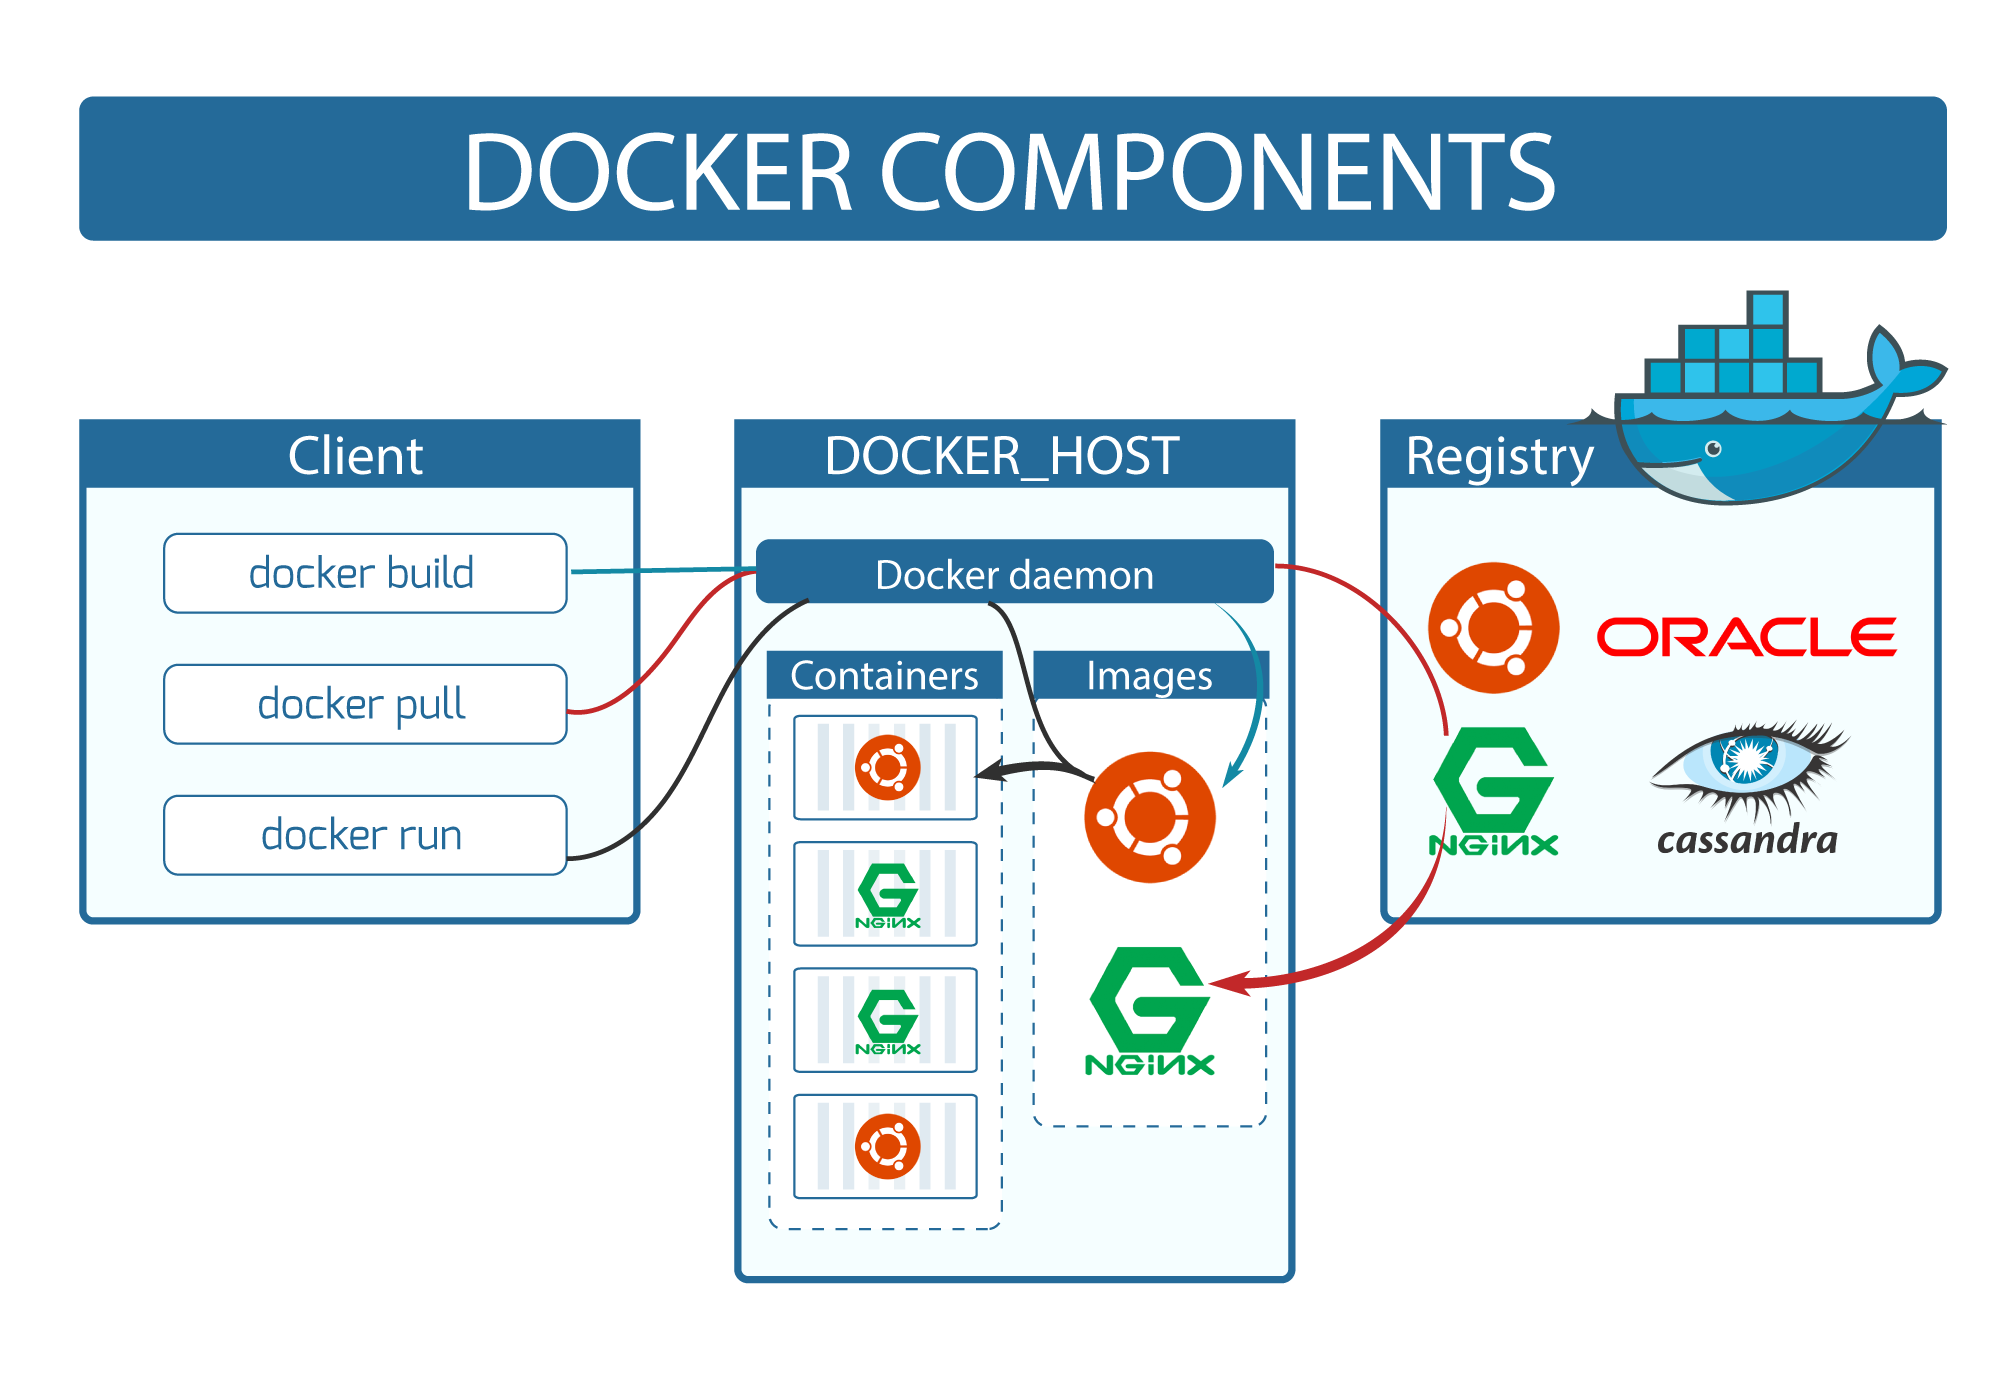
\includegraphics[width=13cm]{obrazky-figures/docker.png}
  \caption{Docker architecture with all its components and commands. Docker can pull or build specific image and then run it in docker container.}
  \label{fig:docker_architecture}
\end{figure}


Since docker is able to run services such as Qpid-dispatch very easily and also allows communication between containers, it is possible to deploy Maestro with proper SUT in containers and analyze behavior in the container network or just run Maestro on single machine. However, for proper performance results we need real machines, so docker containers we used only for Maestro development and trying some basic stuffs with Maestro. The docker architecture is depicted in the Figure \ref{fig:docker_architecture} \cite{Docker-img}.

\section{Qpid-Dispatch Router}
Qpid-Dispatch is a lightweight AMQP message router suitable for building scalable and highly performant messaging networks. This router is an application layer program, w.r.t. ISO/OSI\footnotemark{} model, running either as a normal user program or as a daemon. In particular, it has the following key features:

\begin{itemize}
	\setlength\itemsep{0em}
	\item Connects clients and brokers into an internet-scale messaging network with uniform addressing.
	\item Supports high-performance direct messaging.
	\item Uses redundant network paths to route around failures.
	\item Streamlines the management of large deployments.
\end{itemize}
The following summary of Qpid-Dispatch router was composed based on knowledge available~in~\cite{RH:Interconnect}.

\footnotetext{ISO/OSI\,---\,\url{http://www.studytonight.com/computer-networks/complete-osi-model}}

\subsection{Theory of Operation}
The router accepts AMQP connections from senders and receivers and further creates AMQP connections to Message Brokers or similar AMQP-based services. Through these connections sender is able to reach receiver, which can be another client in the network or a message broker. Note, that the client can exchange messages directly with another client without involving a broker at all. The router classifies all of the incoming messages and routes them between senders and receivers. The router is designed to be deployed in topologies of multiple routers, preferably with redundant paths, to continually provide connectivity in the case any router in the network fails. For routing Qpid-Dispatch uses link-state routing protocols\footnote{Link-state protocols\,---\,\url{https://www.certificationkits.com/cisco-certification/ccna-articles/cisco-ccna-intro-to-routing-basics/cisco-ccna-link-state-routing-protocols/}} and algorithms similar to OSPF or IS-IS to calculate the best path (e.g. the path with the lowest cost) from sender to receiver through the whole network and to recover from failures.

\subsection{Addresses and Connections}
\label{Addresses and Connections}
Qpid-Dispatch is able to connect client servers, AMQP services, and other router implementations through network connections. The router provides multiple components and settings for specifying the service on the other side of connection link as follows:

\begin{description}
	\setlength\itemsep{0em}
	\item \textbf{Addresses\footnotemark{}}\,---\,are used to control the flow of messages across a network of routers. Addresses can specify messages and they are also used during the creation of links since links are bounded to the specific address field of a source and a target. The address can refer to topics or queues that match multiple consumers to multiple producers. There are two types of addresses:
	\begin{itemize}
		\setlength\itemsep{0em}
		\item \textbf{mobile}\,---\,the address is a rendezvous between senders and receivers. The router is then a message distributor.
		\item \textbf{link route}	\,---\,the address is a private messaging path between sender and receiver. The router than only passes messages between end points.
	\end{itemize}
	\item \textbf{Listener}\,---\,is used to accept client connections. Listeners have several types that are defined by their role:
	\begin{itemize}
		\setlength\itemsep{0em}
		\item \textbf{normal}\,---\,the connection is used for AMQP clients using normal message delivery.
		\item \textbf{inter-router}\,---\,the connection is created to only link another router. Inter-router connection can only be established over inter-route listeners.
		\item \textbf{route-container}\,---\,the connection is established to a broker or other resource that holds a known address.
	\end{itemize}
	\item \textbf{Connector}\,---\,is used as an interface for creating a connection with brokers or other AMQP entities using connectors. The same as listeners, connector has several types that are defined by their role:
	\begin{itemize}
		\setlength\itemsep{0em}
		\item \textbf{normal}\,---\,the connection is used for AMQP clients using normal message delivery. The router will initiate the connection but links are created by the peer that accepts the connection.
		\item \textbf{inter-router} and \textbf{route-container}\,---\,they are the same as listener's modes.
	\end{itemize}
\end{description}

\footnotetext{Addresses in this discussion refer to AMQP protocol addresses, not to TCP/IP addresses.}

To ensure the security the router uses the \emph{SSL/TLS (Sockets Layer and Transport Layer Security)}\footnote{SSL\,---\,\url{https://tools.ietf.org/html/rfc6101}; TLS\,---\,\url{https://tools.ietf.org/html/rfc5246}} protocol and its related certificates and \emph{SASL (Simple Authentication and Security Layer)}\footnotemark{} protocol mechanisms to encrypt and authenticate remote peers. Router listeners act as network servers and connectors act as network clients. Both of these components may be configured securely with SSL/TLS and SASL.

\footnotetext{SASL\,---\,\url{https://tools.ietf.org/html/rfc4422}}


\subsection{Message Routing}
\label{Message Routing}
Addresses have semantics associated with them. These semantics control how routers behave when they see the address being used. There are two ways how the router can route messages based on addresses:

\begin{description}
	\setlength\itemsep{0em}
	\item \textbf{Routing pattern}\,---\,defines paths that message with a mobile address can take. These routing patterns can be used in both cases of message delivery; with broker or directly through the router.
	\begin{itemize}
		\setlength\itemsep{0em}
		\item \textbf{Balanced}\,---\,anycast\footnotemark{} method in which multiple receivers are allowed to use the same address.
		\item \textbf{Closest}\,---\,anycast method in which every message is sent along the shortest path to reach the destination.
		\item \textbf{Multicast}\,---\,method in which every receiver with the same address receives the copy of the original message.
	\end{itemize}
	\item \textbf{Routing mechanism}\,---\,defines the path to endpoint from sender to receiver.
	\begin{itemize}
		\setlength\itemsep{0em}
		\item \textbf{Message routed}\,---\,message delivery is done based on the address in message's \emph{to} field. The router checks the destination address of the message and finds the same address in its routing table. The message is then sent to all links with that address.
		\item \textbf{Link routed}\,---\,this method uses the same routing table as Message routing with the difference that the routing occurs during the link-attach operation and link attaches are propagated along the appropriate path to the destination. This results into a chain of links from source to destination.
	\end{itemize}
\end{description}
A~message can be delivered with various degrees of reliability such as \emph{at most once}, \emph{at least once} or \emph{exactly once}.

\footnotetext{Anycast vs. Multicast\,---\,anycast method sends data to every node in network, while multicast method sends data only to specified group of nodes.}

\section{Automatic Topology Generator}
For proper testing of the various messaging systems we need multiple topologies with different components and different settings. However creating and deploying the scenarios manually for each test scenario is rather slow and annoying, even with just a few scenarios. The solution to this problem is divided into two parts: a simple topology generator, which transform metadata, defined by user, into configuration files for each component contained in metadata, and automatic \emph{Ansible} scripts, which deploy the whole topology to actual physical machines. User only has to define is a metadata file, a single file for the whole topology instead of single file for each component, and then start the Ansible script which ensures configuration files generation and the deployment.


\subsection{Topology Components}
Messaging system consists of multiple components with specific roles. In our case, testing topologies will contain clients, brokers, and routers. Clients refer to message senders and receivers, but there is no need for specific configuration for each client at all. Message settings is another case, but Maestro deals with it as was mentioned at Chapter \ref{Messaging Performance Tool}.

\subsubsection*{Broker}
Broker configuration file offers various settings and protocols such as specialized queuing behaviors, message persistence, or manageability. The following list shows selected capabilities of the broker:

\begin{itemize}
	\setlength\itemsep{0em}
	\item \textbf{User access}\,---\,allows guest or authentication access to users.
	\item \textbf{Multiple Protocol Support}\,---\,broker supports AMQP, MQTT, STOMP, OpenWire and Core protocols.
	\item \textbf{Connections}\,---\,can establish connection to another AMQP-based service such as another broker or router.
	\item \textbf{Queues}\,---\,user can specify new queues in configuration file or allow auto-create option.
	\item \textbf{Messaging types}\,---\,refers to approach how to deliver messages, e.g. are point-to-point or publish-subscribe approach.
	\item \textbf{Logging level}\,---\,broker offers the setup for different logging levels.
\end{itemize}
Note, that broker configuration is not implemented yet, but the design of the automatic configuration generation will be shared with router configuration generation.

\subsubsection*{Router}
Similarly to the broker configuration, the router offers various types of configurations. The basics were explained in Subsections \ref{Addresses and Connections} and \ref{Message Routing}, but for better understanding of all capabilities we~recommend to refer to Qpid-Dispatch documentation \cite{RH:Interconnect}.

\subsection{Input and Output Format}
The input format should be user-friendly and easy to update even for large topologies. Hence, as the input we choose one single file (\texttt{config.yml}) in \emph{YAML}\footnotemark{}  language, which is similar to JSON format but is better readable for humans. Topology Generator needs information about all hosts in the topology and which type of topology it should generate. For that purpose there are two attributes in the configuration file; the first is the \emph{inventory path} which refers to the location of \emph{Inventory}\,---\,file, containing all hosts in topology in the specific format (for its specification refer to Appendix \ref{AP:Inventory}). It is a simple configuration file with enumeration of host names and their IP addresses. The other attribute is the type of the topology it should generate. The user can either specify one of the simple types of graph, such as line, circle, or complete, which does not need any other information except Inventory or one can specify path to graph metadata, which are described in Subsection \ref{Graph Metadata} in more details.

On the other hand, the output format should be easy for automatic parsing. The best format for machine parsing in Ansible is JSON or YAML format, since both of them can be loaded with same functions. Output of the generator will be then passed to an Ansible script immediately after the creation without any user intervention. However, user should have option to see the generator output in YAML format, because in case of larger topologies JSON is badly readable. Hence output will be one JSON file with variables for template. Each node from Inventory will have its own variables separated from variables of other nodes. Scheme of the input and output for Topology Generator is shown in the Figure \ref{fig:generator}.

\begin{figure}[H]
  \centering
  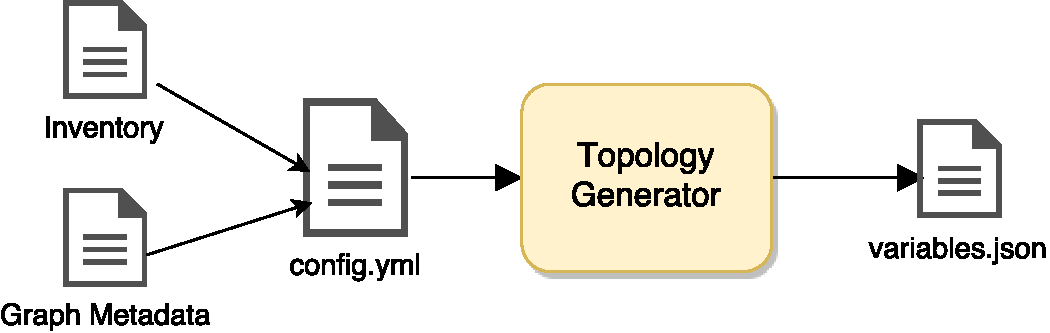
\includegraphics[width=10cm]{obrazky-figures/generator.pdf}
  \caption{Topology generator takes input YAML configuration containing specification of graph metadata and outputs sets of variables in JSON format.}
  \label{fig:generator}
\end{figure}

\footnotetext{YAML - \url{http://docs.ansible.com/ansible/latest/YAMLSyntax.html}}

\subsection{Graph Metadata}
\label{Graph Metadata}
The technology used for the actual implementation of Topology Generator is \emph{NetworkX}, a Python package for creation and manipulation of complex networks. This package offers features for creating graphs, multigraphs, random graph generators, plot created graph, and many more. NetworkX also offers graph import and export in YAML structured file, which is useful as a graph metadata; simple example of file is shown in Appendix \ref{AP:Graph Metadata}.

In these metadata user can specify any setting for each node. For example, user can specify the listener for router\,1, or connector for router\,2 as you can see in the example below.

\begin{verbatim}
---
directed: false
graph: {}
nodes:
- type: router
  id: router1
  listener:
  	- host: 0.0.0.0
  	  port: 1080
  	  role: inter-router
- type: router
  id: router2
  connector:
  	- name: router1
  	  host: router1
  	  port: 5675
  	  role: inter-router
multigraph: false
\end{verbatim}
From these metadata NetworkX creates two nodes with type, id, and listener or connector attributes. These attributes will be used to generate configuration files for each node. All possible attributes that user can specify for each node are available in Appendix \ref{AP:Qpid-Dispatch Configuration File Template}.

However, specifying all attributes of each node is not very user-friendly approach, especially in the case of large topologies. So user can only specify nodes and links between them and generator will add all necessary default attributes in order to establish connection between nodes. The example of this metadata file can be seen in Appendix \ref{AP:Graph Metadata}.

\subsection{Topology Deployment}
Every node specified in the Inventory has to receive proper configuration files for services running on it. This job is handled by the Ansible, since it can connect to all nodes from Inventory and copy configuration files to proper destination folders. Ansible script loads data from Topology Generator and creates configuration files based on loaded variables and the common template for Qpid-Dispatch. The created file will then be sent to the proper node based on node name from Inventory, which has to be same as router name specified in generated variables. The scheme of configuration deployment is depicted in the Figure \ref{fig:deployment}.

\begin{figure}[H]
  \centering
  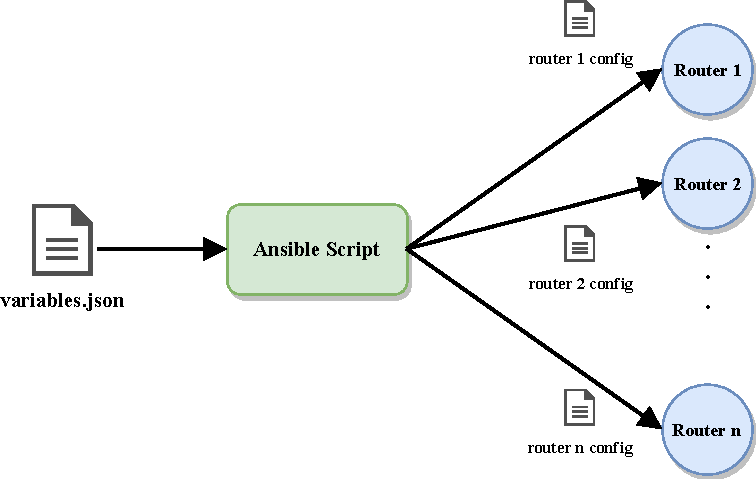
\includegraphics[width=12cm]{obrazky-figures/deployment.pdf}
  \caption{The scheme of configuration files deployment to the nodes The Ansible script takes input file with variables generated by Topology Generator, fills the configurations template and deploy them to corresponding nodes.}
  \label{fig:deployment}
\end{figure}


\section{Agent Performance Module}
The architecture of Maestro (as depicted in the Figure \ref{fig:msg_perf_tool}) originally could not use all performance testing and network recovery possibilities of the Qpid-Dispatch. Hence, for better performance analysis and measurements it was necessary to design and implement additional functionality for Maestro.

In the Figure \ref{fig:msg_perf_tool_update} we show updated version of Maestro architecture. Proper performance testing of router and network analysis with few routers needs special agent, which can manipulate each node. In particular, Maestro should be able to shut down one of the router node and collect data about network behavior during this situation. All these actions will be handled by the new back-end component called \emph{Agent}.

\begin{figure}[H]
  \centering
  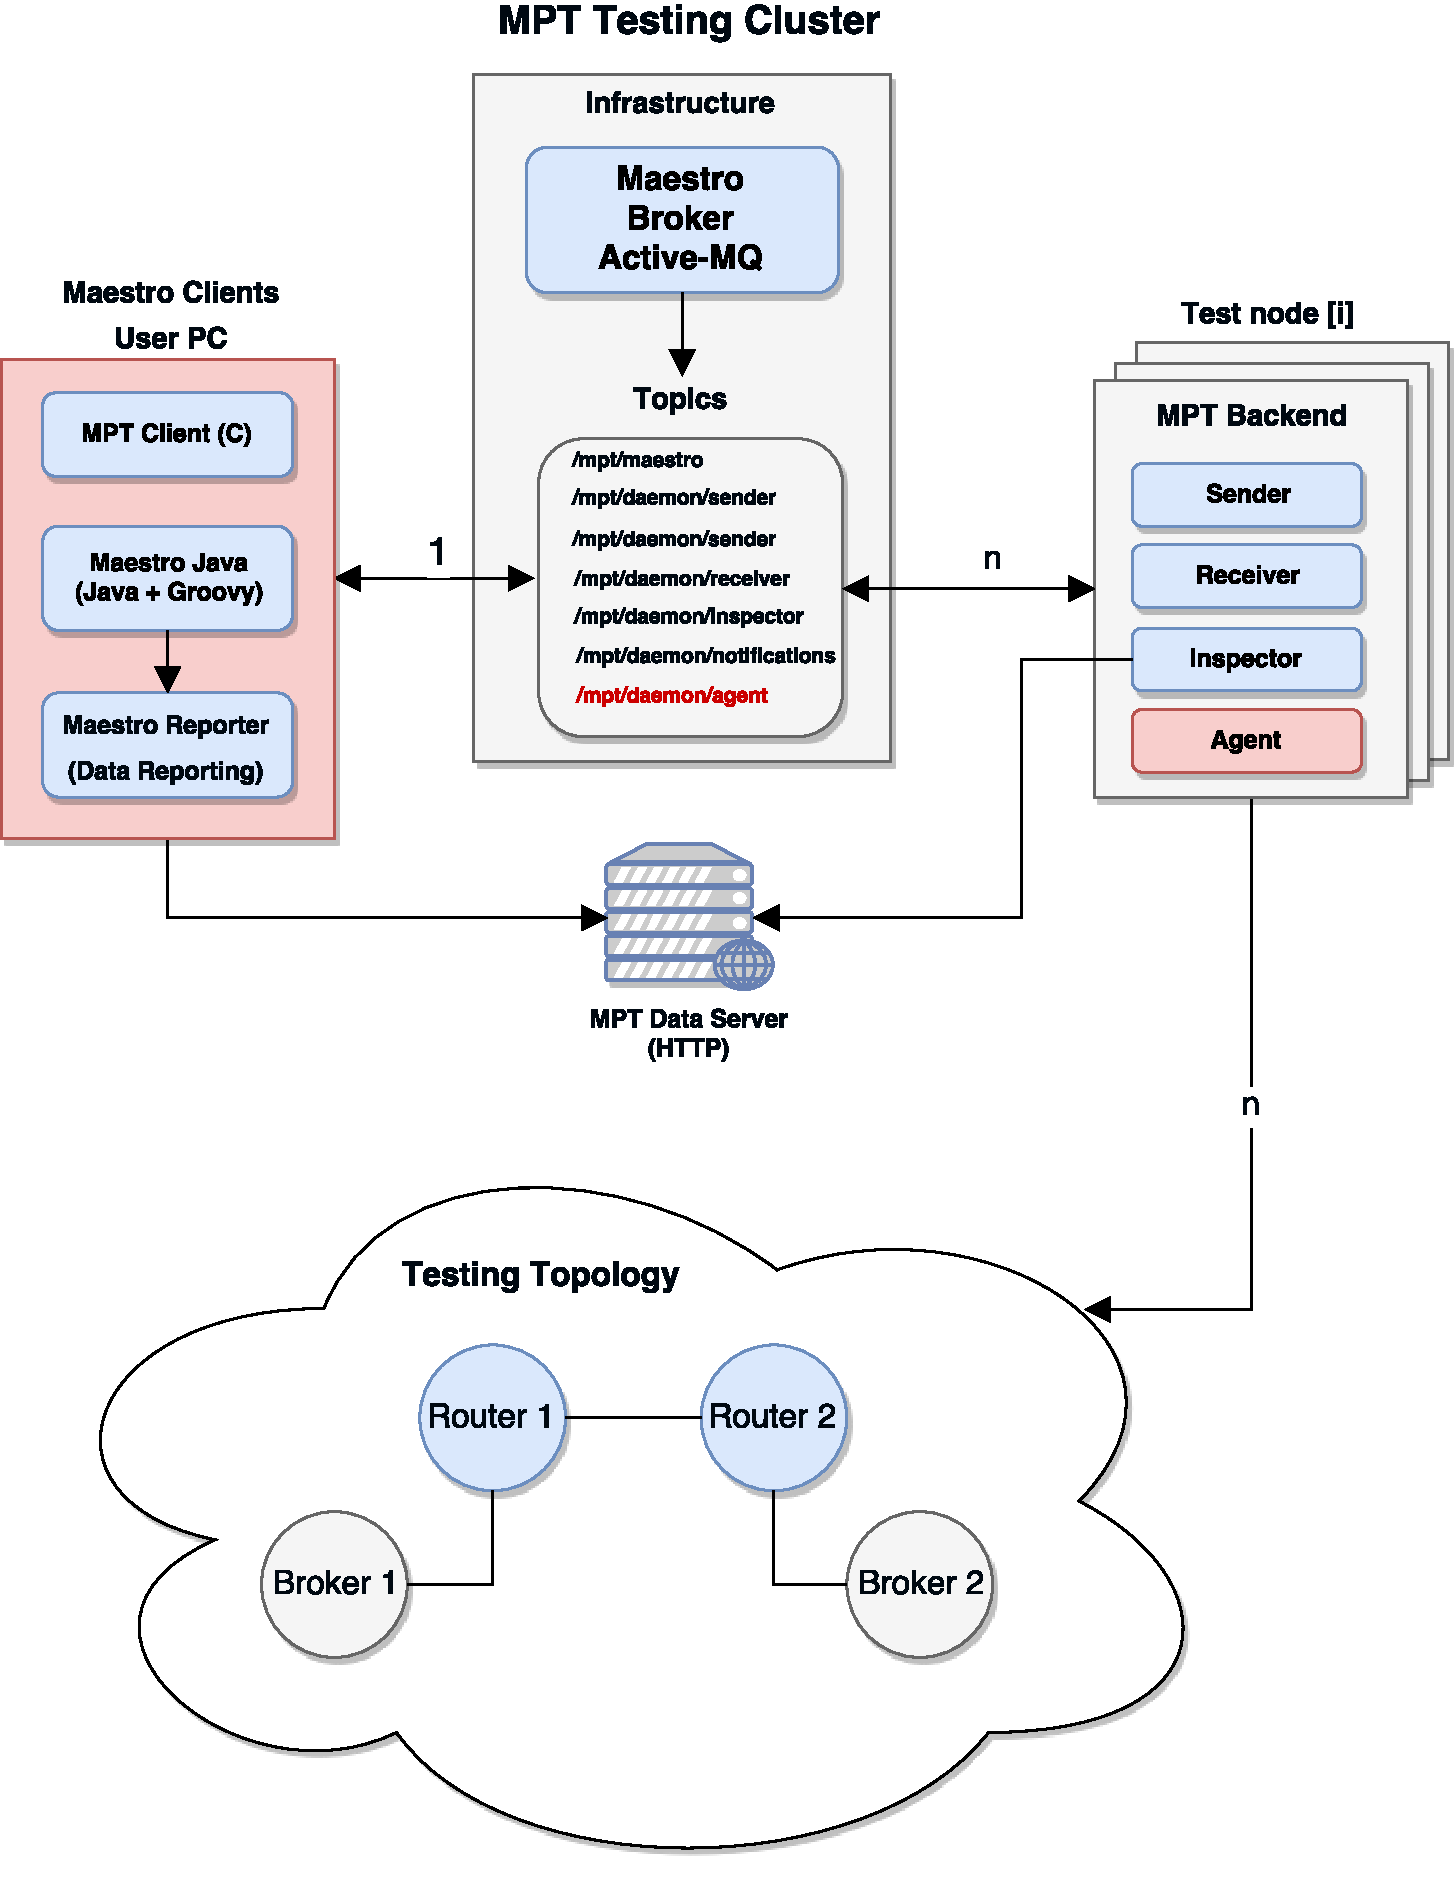
\includegraphics[width=15cm]{obrazky-figures/msg_perf_tool_for_router.pdf}
  \caption{The architecture of updated Maestro for testing of the Qpid-dispatch router.}
  \label{fig:msg_perf_tool_update}
\end{figure}

In the Figure \ref{fig:agent_1} we show the simple scheme of topology with one agent monitoring the router\,2. In this case communication passes through the router\,2 and messages are delivered to receiver without problems. The Figure \ref{fig:agent_2} demonstrates the shutdown of router\,2  by the agent. In that case, the network will choose the redundant link through router\,3 in order to pass messages. This scenario can then answer the question \emph{How does router shutdown influence the latency between sender and receiver?}

\begin{figure}[H]
	\centering
	\begin{minipage}{6.5 cm}
		\subfloat[Network with router agent.\label{fig:agent_1}]{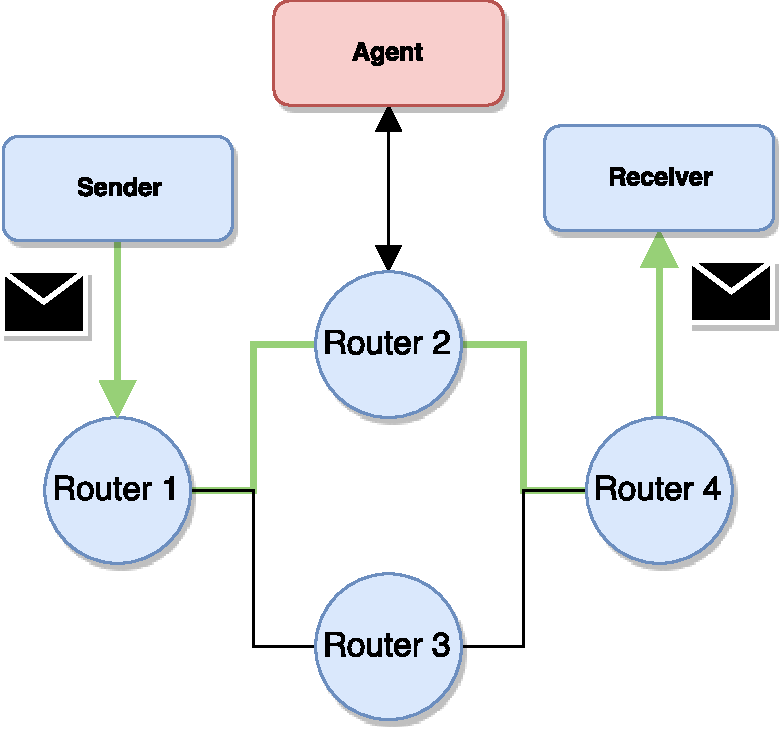
\includegraphics[width=1\linewidth]{obrazky-figures/agent_1.pdf}}
	\end{minipage}
	\begin{minipage}{6.5 cm}
		\subfloat[Router shut-down demonstration.\label{fig:agent_2}]{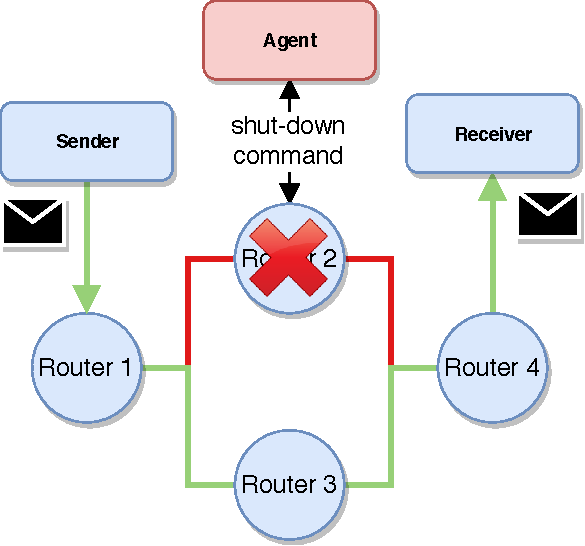
\includegraphics[width=1\linewidth]{obrazky-figures/agent_2.pdf}}
	\end{minipage}
	\caption[A simple network with active router agent.]{A simple network with demonstration of router shut-down.}\label{fig:agent}
\end{figure}

Communication between cluster back-end and user client is realized through Maestro Broker and so for proper message distribution a new topic has to be added. As was mentioned in Section \ref{Collected Data Format}, Maestro Clients communicate with back-end via specialized commands. Router Agent will accept a new set of specialized commands for router control. This set has to be added to existing Maestro Clients. All additional components or components that required update are highlighted by red color in the Figure \ref{fig:msg_perf_tool_update}. The example of simple testing topology consisting of two routers and two brokers is also included in the Figure \ref{fig:msg_perf_tool_update}.


\subsection{Extension Points}
\label{Extension Points}
After although research and discussion with engineers we decided to develop the agent as a service with dynamic command execution, which will be able to run any specific code. At the begging of the test, the agent will receive the command to download a repository with specific scripts serving as an action handlers. The path to repository will be the payload of one of the new commands. After that, the agent will listen on the Maestro Broker and wait for user's command to execute. This command will transport the name of the handler script as a payload of the Maestro's note. The agent will then execute script from payload as an action on the node. In particular, the router restart handler can be part of the downloaded repository and then can be performed after receiving user commands with payload \emph{\"requests/router\_restart.groovy\"}. This functionality makes the agent dynamic, and offers the user an ability execute any specific action he wants.


\subsection{Communication with Agent}
\label{Communication with Agent}
For the communication inside Maestro testing cluster we use the Maestro Protocol, which was described in the Subsection \ref{Communication Between Components}. Maestro Clients have to know how to communicate with this new component in the cluster and so it is necessary to add new communication commands. The following lists new commands which should be added:

\begin{itemize}
	\setlength\itemsep{0em}
	\item \textbf{MAESTRO\_NOTE\_START\_AGENT (18)}\,---\,start the agent service.
	\item \textbf{MAESTRO\_NOTE\_STOP\_AGENT (19)}\,---\,stop the agent service.
	\item \textbf{MAESTRO\_NOTE\_AGENT\_SOURCE (21)}\,---\,set path to user commands handlers.
	\item \textbf{MAESTRO\_NOTE\_USER\_COMMAND (30)}\,---\,execute user's specific command.
\end{itemize}

\subsection{AMQP Inspector}
\label{AMQP Inspector}
The important part of the performance testing are measurements of internal metrics of SUT. Maestro offers Maestro Inspector for this kind of measurements. However, the current version can monitor only Broker, because Inspector is implemented for the specific interface provided by the Broker. Since Broker is written in Java and provides access to JMX\footnote{JMX\,---\,\url{http://www.oracle.com/technetwork/articles/java/javamanagement-140525.html}} via Jolokia\footnote{Jolokia\,---\,\url{https://jolokia.org/}}, we cannot use current implementation of the Inspector for the Qpid-Dispatch as well. The router offers \emph{AMQP management} for interaction with the router on the fly, which is different than Jolokia access. The Jolokia access is based on HTTP/JSON format message exchange between requester and SUT, while AMQP Management is based on AMQP messages with specific format.

The router offers the following information after proper AMQP request to an opened up listener with specific properties:

\begin{itemize}
	\setlength\itemsep{0em}
		\item \textbf{name}\,---\,this property is always set to string property \textbf{self}, which refers to itself object.
		\item \textbf{operation}\,---\,AMQP management offers classic CRUD operations. For inspect message we will always use the option called \textbf{QUERY}.
		\item \textbf{type}\,---\,this property represents the interior package which will parse the request. We will use \textbf{org.amqp.management}.
		\item \textbf{entityType}\,---\,this property is configurable. We use there several options with prefix \textbf{org.apache.qpid.dispatch.} based on the request purpose. The options for request are:
		\begin{itemize}
			\setlength\itemsep{0em}
			\item \emph{router}\,---\,general informations about the router.
			\item \emph{router.stats}\,---\,detailed informations about the router.
			\item \emph{router.link}\,---\,informations about route links.
			\item \emph{router.node}\,---\,general informations about neighbour nodes.
			\item \emph{router.address}\,---\,informations about addresses on the router.
			\item \emph{connector}\,---\,informations about connections.
			\item \emph{allocator}\,---\,informations about memory metrics.
			\item \emph{config.autolink}\,---\,informations about created auto links.
			\item \emph{config.linkRoute}\,---\,informations about created link routes.
		\end{itemize}
		\item \textbf{body}\,---\,message payload, which is usually an empty list. Exceptions are auto links and link routes requests, which needs additional information in the body.
\end{itemize}

\subsubsection*{Collected Data}
\label{Collected Data}
Data collected by the AMQP Inspector are different than those collected by current version of Inspector. After the discussion, we decided to collect data about \emph{general statistics}, \emph{router links} and \emph{memory}. Note, that each data set has multiple data columns, which are all available in Appendix \ref{AMQP Inspector Data Sets}. The following describes the most important data collected by the AMQP Inspector:

\begin{itemize}
	\setlength\itemsep{0em}
	\item \textbf{Timestamp}\,---\,the date and time for the data sample in the format YYYY-MM-DD hh:mm:ss using the W3C defined standard for datetime.
	\item \textbf{General Statistics}\,---\,basic informations about the router such as its active connections, addresses, auto links, accepted messages and etc.
	\begin{itemize}
		\setlength\itemsep{0em}
		\item \textbf{Address Count}\,---\,number of active addresses at current time.
		\item \textbf{Connections Count}\,---\,number of active connections at current time.
	\end{itemize}
	\item \textbf{Router Links}\,---\,informations about all router links which were opened to the router.
	\begin{itemize}
		\setlength\itemsep{0em}
		\item \textbf{Accepted Message Count}\,---\,number of accepted messages at current time.
		\item \textbf{Delivered Message Count}\,---\,number of delivered messages at current time.
		\item \textbf{Released Message Count}\,---\,number of released messages at current time.
		\item \textbf{Undelivered Message Count}\,---\,number of undelivered messages at current time.
	\end{itemize}
	\item \textbf{Memory Statistics}\,---\,informations about allocated memory by the router.
	\begin{itemize}
		\setlength\itemsep{0em}
		\item \textbf{Total Allocated Memory}\,---\,total allocated memory.
		\item \textbf{Memory Allocated by Threads}\,---\,total memory allocated by threads.
	\end{itemize}
\end{itemize}

Each data set is then converted to a line chart, which represents collected values for each request. Data collected by senders and receivers remains the same as in the current version of Maestro.
